\documentclass[conference]{IEEEtran}
\IEEEoverridecommandlockouts
% The preceding line is only needed to identify funding in the first footnote. If that is unneeded, please comment it out.
\usepackage{cite}
\usepackage{amsmath,amssymb,amsfonts}
\usepackage{algorithmic}
\usepackage{graphicx}
\usepackage{textcomp}
\usepackage{xcolor}
\usepackage{gensymb}
\usepackage{listings}
\usepackage[framed,numbered,autolinebreaks,useliterate]{mcode}
\def\BibTeX{{\rm B\kern-.05em{\sc i\kern-.025em b}\kern-.08em
    T\kern-.1667em\lower.7ex\hbox{E}\kern-.125emX}}
\begin{document}

\title{RBE 501 Week 6: Physics by EL Assignment}

\author{\IEEEauthorblockN{Arjan Gupta}
\IEEEauthorblockA{\textit{Robotics Engineering} \\
\textit{Worcester Polytechnic Institute}\\
Worcester, MA, USA \\
agupta11@wpi.edu}
}

\maketitle

\begin{abstract}
This document provides an in-depth solution for the Week 6 Physics by Euler-Lagrange problems in RBE 501.\\
\end{abstract}

\begin{IEEEkeywords}
physics, euler-lagrange equations
\end{IEEEkeywords}

\section{Introduction}
For Week 6, we are given two problems. The first problem shows us a mass $m$ that is free to
move on the surface of a frictionless table. Mass $m$ is attached to another mass $M$ via a
string that goes through a hole in the table. We can assume the string has no spring-like
properties, and is therefore always taut. The representation of this system is shown in 
Figure~\ref{problem-1-given-fig}. Our first objective in this problem is to solve for the Euler-Lagrange
equations of this system with respect to $r$ and $\theta$. Our second and third objectives here
are to discuss the behaviors of $r$ and $\theta$ in the EL equations. The fourth objective of the
first problem is to give the conditions under which $\dot{r}$ and $\ddot{r}$ cause a circular motion
for mass $m$.\\

\begin{figure}[h!]
    \centering
    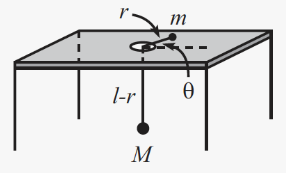
\includegraphics[scale=0.35]{problem-1-given-fig.png}
    \caption{Given figure for Problem 1}
    \label{problem-1-given-fig}
\end{figure}

The second problem shows a mass $m$ that is held at rest on ramp of mass $M$. The ramp has inclination
$\theta$, as shown in Figure \ref{problem-2-given-fig}. The surface of the ramp is frictionless, and the
surface upon which the ramp rests is also frictionless. Our objective is to find the acceleration of
the ramp caused by the release of mass $m$, and we must use Euler-Lagrange approach for this.

\begin{figure}
    \centering
    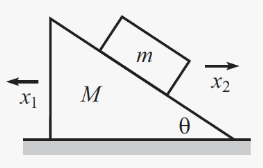
\includegraphics[scale=0.35]{problem-2-given-fig.png}
    \caption{Given figure for Problem 2}
    \label{problem-2-given-fig}
\end{figure}

\section{Materials and Methods}

\subsection{Approach for Problem I}

Our first step toward solving Problem I is to find the overall kinetic energy ($T$) and
overall potential energy ($U$) of the system. We then find the Lagrangian of the system
as $L \equiv T - U$. We can then use the Euler-Lagrangian equation,

\begin{equation} \label{prob1_eq_motion_r}
    \frac{d}{dt} \left(\frac{\partial L}{\partial \dot{r}}\right) = \frac{\partial L}{ \partial r}
\end{equation}
and
\begin{equation} \label{prob1_eq_motion_theta}
    \frac{d}{dt} \left(\frac{\partial L}{\partial \dot{\theta}}\right) = \frac{\partial L}{ \partial \theta}
\end{equation}

to discuss the behaviors of $r$ and $\theta$.\\

\subsubsection{Find overall kinetic energy of the system ($T$)}
In Fig. 1, we consider vector $\textbf{r}$. Say the \textit{x-y} plane is the surface
of the table. Since we consider an angle $\theta$ as shown, we can say,

\[
    \textbf{r} =
    \begin{pmatrix}
        r \cos \theta\\
        r \sin \theta
    \end{pmatrix}
\]

Where the magnitude of $r$ is dependent on theta. Differentiating
with respect to $\theta$ to get velocity,

\[
    \dot{\textbf{r}} =
    \begin{pmatrix}
        \dot{r} \cos \theta - r \dot{\theta} \sin \theta\\
        \dot{r} \sin \theta + r \dot{\theta} \cos \theta
    \end{pmatrix}
\]

To find the kinetic energy, we need the square of this velocity,
which is simply the dot product of the vector with itself.

\begin{align*}
    \dot{\textbf{r}}^2 = \dot{\textbf{r}} \cdot \dot{\textbf{r}}
    =&~(\dot{r} \cos \theta - r \dot{\theta} \sin \theta)^2 +
    (\dot{r} \sin \theta + r \dot{\theta} \cos \theta)^2\\
    =&~\dot{r}^2 \cos^2 \theta + r^2 \dot{\theta}^2 \sin^2 \theta 
    + 2 r \dot{r} \dot{\theta} \cos\theta \sin\theta + \\
    &~\dot{r}^2 \sin^2 \theta + r^2 \dot{\theta}^2 \cos \theta
    - 2 r \dot{r} \dot{\theta} \cos\theta \sin\theta\\
    =&~\dot{r}^2 (\cos^2\theta + \sin^2\theta) 
    + r^2\dot{\theta}^2 (\cos^2\theta + \sin^2\theta)\\
\end{align*}
Hence,
\[
    \dot{\textbf{r}}^2 = \dot{r}^2 + r^2\dot{\theta}^2
\]

Therefore the kinetic energy of the mass $m$ moving on the table is given as,

\begin{equation} \label{prob1_ke_mass_small_m}
    T_m = \frac{1}{2}~m~(\dot{r}^2 + r^2\dot{\theta}^2)
\end{equation}
Also, the length of the string that suspends 
mass $M$ is $l-r$, where
total length of the string is $l$. The suspended part
of the string is also along the axes perpendicular to the table,
which is the \textit{z} axis. Therefore, the kinetic energy of the
mass $M$ moving perpendicular to the table is given as

\begin{equation} \label{prob1_ke_mass_big_m}    
    T_M = \frac{1}{2}~M~\left(\frac{d}{dt}(l-r)\hat{\textbf{z}}\right)^2 = \frac{1}{2}~M~\dot{r}^2
\end{equation}

So, using Equations~\ref{prob1_ke_mass_small_m} and~\ref{prob1_ke_mass_big_m},
the total kinetic energy of the system ($T$) is,

\begin{align*}
    T &= T_m + T_M\\
      &=\frac{1}{2}~m~(\dot{r}^2 + r^2\dot{\theta}^2) + \frac{1}{2}~M~\dot{r}^2
\end{align*}
Rearranging,
\begin{equation} \label{prob1_overall_ke}
    T = \frac{1}{2} \dot{r}^2 (m + M) + \frac{1}{2} m r^2 \dot{\theta}^2
\end{equation}

\subsubsection{Find overall potential energy of system}
The potential energy is also a sum of the potential energies of the masses
$m$ and $M$ in the system. The only source of potential energy in
this system is gravity caused by the earth. Since we are free to define
the reference point from where we can count the height from earth, let us
define the table-top in Figure~\ref{problem-1-given-fig} as height $h = 0$.
Also, $g$ is the constant acceleration due to gravity.

This means,

\[
    U_m = mgh = mg~(0) = 0
\]

and,

\[
    U_M = Mg(-(l-r)) = Mg(r-l)
\]

So, the overall potential energy of the system is simply,
\begin{equation} \label{prob1_overall_pe}
    U = U_M + U_m = Mg(r-l)
\end{equation}

\subsubsection{Find Lagrangian of the system}
The Lagrangian of the system is given as $L \equiv T - U$. Using Equations 
\ref{prob1_overall_ke} and \ref{prob1_overall_pe}, we get

\begin{align*}
    L &= \left(\frac{1}{2} \dot{r}^2 (m + M) + 
        \frac{1}{2} m r^2 \dot{\theta}^2\right)-Mg(r-l)\\
    L &= \frac{1}{2} \dot{r}^2 (m + M) + 
    \frac{1}{2} m r^2 \dot{\theta}^2 - Mg(r-l)
\end{align*}

\subsubsection{Find equations of motion for the system}
We can use Equations \ref{prob1_eq_motion_r} and \ref{prob1_eq_motion_theta}
to find the equations of motion.\\

For the equations of motion with respect to $r$, we have,

\begin{equation}\label{prob1_el_sol1}
    \frac{\partial L}{\partial r} = m~r~\dot{\theta}^2 - Mg
\end{equation}
\begin{equation}\label{prob1_el_sol2}
    \frac{d}{dt}\left(\frac{\partial L}{\partial \dot{r}}\right) 
    = \frac{d}{dt}\left( \dot{r}(m + M) \right) = \ddot{r}(m + M)
\end{equation}\\

And for the equations of motion with respect to $\theta$, we have,

\begin{equation}\label{prob1_el_sol3}
    \frac{\partial L}{\partial \theta} = 0
\end{equation}
\begin{equation}\label{prob1_el_sol4}
    \frac{d}{dt}\left(\frac{\partial L}{\partial \dot{\theta}}\right) 
    = \frac{d}{dt}\left( m~r^2~\dot{\theta} \right)
\end{equation}

While it is possible to show the expanded differentiated form of 
Equation~\ref{prob1_el_sol4}, we have left it as is in order
to aid our Discussion better.

\subsubsection{Circular motion conditions}

Problem 1 also asks to set the conditions under which mass $m$
has circular motion, by setting
$\dot{r} = 0$ and $\ddot{r} = 0$. We substitute these values in Equations~\ref{prob1_el_sol1}
and~\ref{prob1_el_sol2}. Also, we set $r = r_{circ}$ and $\dot{\theta} = \omega_{circ}$.
This gives us the following,

\begin{align*}
    m~r_{circ}~{\omega_{circ}}^2 - Mg &= (0) (m + M)\\
    m~r_{circ}~{\omega_{circ}}^2 - Mg &= 0\\
    m~r_{circ}~{\omega_{circ}}^2 &= Mg
\end{align*}
So, we can write $r_{circ}$ as,
\begin{equation}\label{r_circ_val}
    r_{circ} = \frac{Mg}{m{\omega_{circ}}^2}
\end{equation}

Also, under these conditions, we set Equations~\ref{prob1_el_sol3} and~\ref{prob1_el_sol4}
with $\dot{\theta} = \omega_{circ}$ and $r = r_{circ}$ as follows,

\begin{align*}
    \frac{d}{dt}\left( m~{r_{circ}}^2~\omega_{circ} \right) &= 0\\
    \int \left[ \frac{d}{dt}\left( m~{r_{circ}}^2~\omega_{circ} \right) \right] dt &= \int (0) dt
\end{align*}
Which gives the well-known physical fact that angular momentum remains preserved in this system,
\begin{equation}
    m~{r_{circ}}^2~\omega_{circ} = C_{am}
\end{equation}
This is because the standard formula of the angular momentum, $mvr$, can
easily be rewritten as $mr^2\omega$ because velocity is $r\omega$. We have
chosen $C_{am}$ to denote the constant angular momentum of the system.
Futhermore, we can write $\omega_{circ}$ as,
\begin{equation}\label{omega_circ_val}
    \omega_{circ} = \frac{C_{am}}{m~{r_{circ}}^2}
\end{equation}

We can now substitute~\ref{omega_circ_val} into~\ref{r_circ_val},

\begin{align*}
    r_{circ} &= \frac{Mg(m~{r_{circ}}^2)^2}{m~{C_{am}}^2}\\
    r_{circ} &= \frac{Mg~m^2~r_{circ}^4}{m~{C_{am}}^2}\\
    1 &= \frac{Mg~r_{circ}^3}{{C_{am}}^2}
\end{align*}
Isolating $r_{circ}$,
\begin{equation}\label{prob1_obj4_r}
    r_{circ} = \sqrt[3]{\frac{{C_{am}}^2}{mMg}}
\end{equation}

Additionally we can substitute~\ref{r_circ_val} into~\ref{omega_circ_val}.
\begin{align*}
    \omega_{circ} &= \frac{C_{am}(m{\omega_{circ}}^2)^2}{m~{(Mg)}^2}\\
    \omega_{circ} &= \frac{C_{am}m^2{\omega_{circ}}^4}{m~M^2g^2}\\
    1 &= \frac{C_{am}~m~{\omega_{circ}}^3}{M^2g^2}\\
\end{align*}
Isolating $\omega_{circ}$,
\begin{equation}\label{prob4_obj4_omega}
    \omega_{circ} = \sqrt[3]{\frac{M^2g^2}{m~C_{am}}}
\end{equation}

\subsection{Approach for Problem 2}

\subsubsection{Restate objective in technical terms}
Like Problem 1, we first find $T$ and $U$ in order to give us
$L \equiv T - U$. After that we solve for the following
equations of motion,

\begin{equation} \label{prob2_eq_motion_x1}
    \frac{d}{dt} \left(\frac{\partial L}{\partial \dot{x_1}}\right) = \frac{\partial L}{ \partial x_1}
\end{equation}
and
\begin{equation} \label{prob2_eq_motion_x2}
    \frac{d}{dt} \left(\frac{\partial L}{\partial \dot{x_2}}\right) = \frac{\partial L}{ \partial x_2}
\end{equation}

Where $x_1$ and $x_2$ are the displacements as shown in Figure~\ref{problem-2-given-fig}.

\subsection{Find overall kinematic energy of system}

Let us first establish our vectors. As shown in the diagram, 

\section{Results}

\subsection{Results for Problem 1}

Our first objective of Problem 1 was to find the equations of motion in terms
of $r$ and $\theta$. From Equations~\ref{prob1_el_sol1},~\ref{prob1_el_sol2},~\ref{prob1_el_sol3},~\ref{prob1_el_sol4}, these are as follows,\\

\begin{equation}\label{prob1_result_el1}
    \boxed{
        m~r~\dot{\theta}^2 - M~g~l = \ddot{r}~(m + M)
    }
\end{equation}

and,

\begin{equation}\label{prob1_result_el2}
    \boxed{
        \frac{d}{dt}\left( m~r^2~\dot{\theta} \right) = 0
    }
\end{equation}

Our second and third objectives were to discuss Equations~\ref{prob1_result_el1},~\ref{prob1_result_el2},
which we will do in our next section. The results of the fourth objective, by using~\ref{prob1_obj4_r}
and~\ref{prob4_obj4_omega}, are as follows,

\begin{equation}
    \boxed{r_{circ} = \sqrt[3]{\frac{{C_{am}}^2}{mMg}}}
\end{equation}

and,

\begin{equation}
    \boxed{\omega_{circ} = \sqrt[3]{\frac{M^2g^2}{m~C_{am}}}}
\end{equation}

Where $C_{am}$ is the constant angular momentum conserved for $r_{circ}$ and $\omega_{circ}$,
which are the radius and angular velocity values when the linear velocity and linear acceleration with
regards to the vector $\textbf{r}$ are 0.

\subsection{Result for Problem 3--5}

For Problem 2, we obtained the following results.

\section{Discussion}

It was a great exercise the solve this week's problem set, and the author thanks
the Professor for this.
\bibliography{refs.bib}
\bibliographystyle{IEEEtran}

\end{document}